\chapter{Evaluation}
Ziel der Evaluation ist es zu prüfen, ob der implementierte GDB-Stub eine grundlegende Debugging-Sitzung mit D3OS ermöglicht. Dazu werden die implementierten Befehle des Stubs mithilfe von Testfunktionen, die in separaten Kernel-Threads aufgerufen werden, getestet. In den Testfunktionen werden lokale Variablen, weitere Funktionsaufrufe, Schleifen und Objektinstanzen verwendet. Die Tests wurden sowohl in einer emulierten Umgebung, als auch auf echter Hardware durchgeführt. D3OS wurde mit Debuginformationen kompiliert. Dazu wurde der Befehl \texttt{cargo make --no-workspace gdbstub} verwendet.

\section{Breakpoints}
Die Tests haben gezeigt, dass Software Breakpoints gesetzt, getroffen und entfernt werden können. Aktuell funktioniert das jedoch nur im Kernel-Space und nur auf Funktionen, die nicht in den Exception-Handlern aufgerufen werden, da der Breakpoint dort sonst erneut getroffen wird, bevor er entfernt werden kann, was zu einer unendlichen Schleife führt. Um Software Breakpoints auch im User-Space verwenden zu können, muss der Adressraum des jeweiligen Prozesses geladen werden. Hardware Breakpoints lassen sich jedoch auch im User-Space setzen. Außerdem kann es vorkommen, dass GDB mehrere Software Breakpoints auf die gleiche Zeile setzt. Bei Makro Aufrufen kann es sein, dass eine Zeile im Quellcode mehreren Adressen zugeordnet ist. Dann setzt GDB auf jeder der Adressen einen Breakpoint und trifft diese nacheinander.

\section{Single-Stepping}
Single-Stepping wurde durch die Befehle \texttt{step} und \texttt{next} nach einem getroffenen Breakpoint getestet. Dabei zeigte sich, dass Single-Stepping größtenteils so wie erwartet funktioniert. Man kann jedoch kein Step Into in Funktionen durchführen, die durch die Exception Handler des Stubs aufgerufen werden. Da GDB das Step Into durch temporäre Software Breakpoints realisiert, wird bei solchen Funktionen, wie zum Beispiel dem statischen Scheduler Aufruf, eine unendliche Exceptionschleife ausgelöst. GDB will in die Funktion eintreten und setzt einen Breakpoint auf die Funktion. Das Programm trifft den Breakpoint und betritt den Handler. Der Handler ruft aber ebenfalls die Funktion auf, während der Breakpoint noch aktiv ist, wodurch er wieder getroffen wird und der Handler neu betreten wird. Um nicht aktiv darauf achten zu müssen bestimmte Funktionen zu überspringen, bietet GDB den \texttt{skip} Befehl an \cite{gdb}. Dadurch lassen sich bestimmten Funktionen und auch ganze Dateien von einem Step Into ausschließen. Dazu muss der vollständige Pfad angegeben werden. Der Scheduler Aufruf aus der lib.rs Datei lässt sich zum Beispiel durch \texttt{skip -rfu kernel::scheduler} überspringen. Bei Makros ist das ganze jedoch schwieriger, weil nicht der Name des Makros verwendet werden kann, sondern die Funktionen des expandierten Makrocodes verwendet werden müssen. Das \texttt{info!()} Makro lässt sich zum Beispiel durch den Befehl \texttt{skip -rfu .*log::.*} überspringen. Dadurch überspringt GDB alle Funktionen, deren Name \texttt{log} beinhaltet.\\
Single-Stepping von einem Hardware Breakpoint im User-Space funktioniert jedoch nicht, da dafür wieder der Adressraum geladen sein muss.

\section{Registerzugriff}
Da viele der anderen Funktionen auf den Registerwerten basieren, müssen diese nicht isoliert getestet werden. Solange Single-Stepping und Speicherzugriffe korrekt funktionieren, werden auch die Register korrekt ausgelesen.

\section{Speicher auslesen}
Sowohl lokale Variablen, als auch Instanzen von Structs und deren Felder lassen sich auslesen. Die Zugriffe liefern jedoch nur das erwartete Ergebnis, wenn auch die Registerzustände korrekt ausgelesen werden und der Adressraum geladen ist. 

\section{Probleme des Serial Ports}
D3OS verwendet für die Implementierung des Loggers ebenfalls den seriellen Port. Da die Bildungsrechner, auf denen getestet wurde, nur einen solchen Anschluss haben, führt das dazu, dass der Stub und die Logger sich Ressourcen teilen müssen. Damit der Stub und GDB sich zuverlässig austauschen können, müssen alle Logger ausgeschaltet sein und die Zuweisung des \texttt{ComPorts} im Konstruktor des Loggers muss ebenfalls auskommentiert sein. Wird das nicht gemacht, kann es zu unerwartetem Verhalten kommen. Dabei kann es sein, dass der Stub entweder falsche Paketet an GDB schickt und dadurch ein Error ausgelöst wird oder die Pakete, die von GDB verschickt werden, fehlerhaft ankommen, weil eine andere Komponente mit Zugriff auf den seriellen Port die Bytes konsumiert. Dieses Problem tritt in der emulierten Umgebung mit QEMU nicht auf, da dort in der Konfigurationsdatei mehrere serielle Anschlüsse eingestellt werden können.\\
Auf der neusten Version von D3OS reicht das aber auch nicht aus. Dort werden scheinbar trotzdem fehlerhafte Pakete ausgetauscht, obwohl alle Instanzen, die einen seriellen Port nutzen, ausgeschaltet oder auskommentiert sind. Durch die Debug-Ausgaben von GDB kann man beobachten, dass der Stub standardmäßig im \texttt{noack Mode} läuft. Das bedeutet, dass nach dem initialen Verbindungsaufbau keine \texttt{ACK-Pakete} mehr ausgetauscht werden. Wenn man diesen auf der neusten Version aber ausschaltet, kann man sehen, dass statt der \texttt{ACK-Pakete} teilweise Bytes oder auch ganze Pakete vom Stub an GDB zurückgeschickt werden. Der serielle Port verarbeitet also fehlerhaft die Pakete, was entweder zu einem \texttt{UnexpectedHeader} Fehler beim Verbindungsaufbau oder einem \texttt{MismatchedChecksum} Fehler während der Benutzung führt. Beim testen konnte nicht rausgefunden werden, was genau dieses Verhalten auslöst.


\begin{figure}[h]
  \centering
  \begin{subfigure}[b]{0.4\textwidth}
    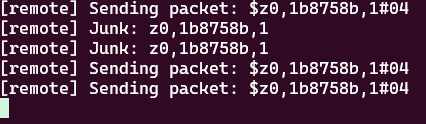
\includegraphics[width=1.0\linewidth]{img/echo}
  \end{subfigure}
  \caption{Stub schickt Pakete zurück}
  \label{grafik_echo}
\end{figure}

\begin{figure}[h]
  \centering
  \begin{subfigure}[b]{1.0\textwidth}
    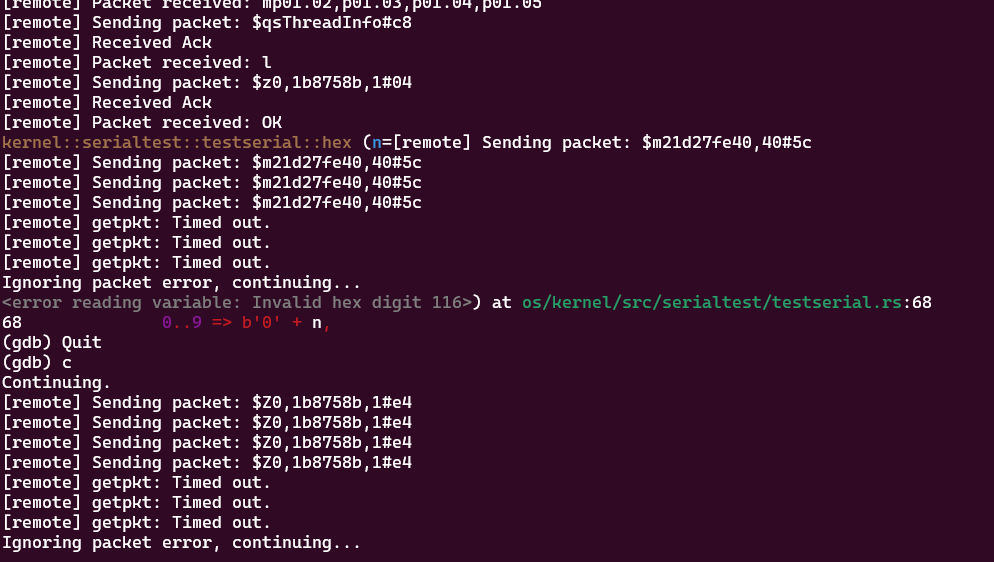
\includegraphics[width=1.0\linewidth]{img/timeout}
  \end{subfigure}
  \caption{Timeout}
  \label{grafik_timeout}
\end{figure}

\begin{figure}[H]
  \centering
  \begin{subfigure}[b]{1.0\textwidth}
    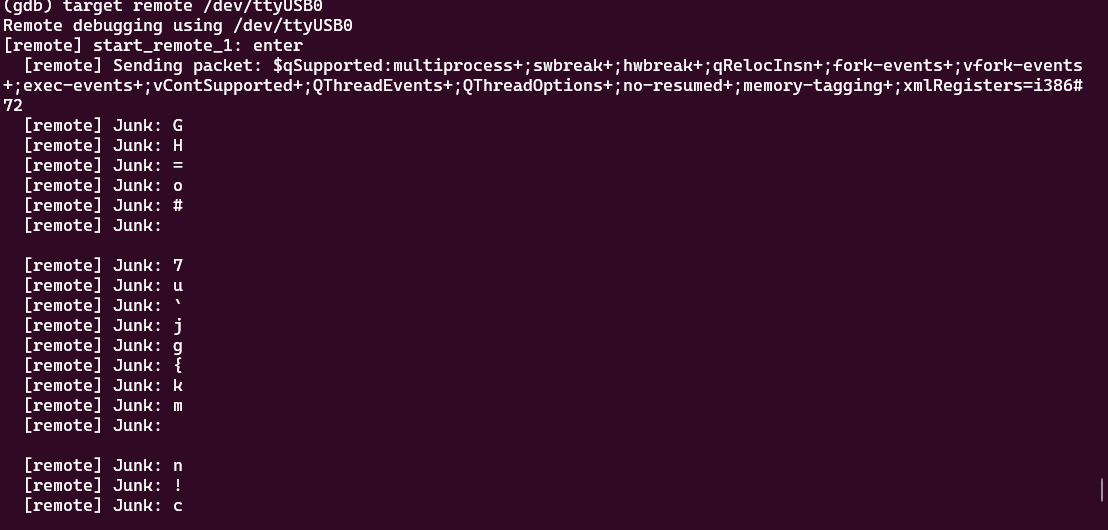
\includegraphics[width=1.0\linewidth]{img/unexpected_header}
  \end{subfigure}
  \caption{Unexpected Header}
  \label{grafik_header}
\end{figure}


\section{Grenzen der Implementierung}
Die aktuelle Implementierung ermöglicht die grundlegenden Debugging-Funktionen im Kernel-Space, besitzt jedoch folgende Einschränkungen:
\begin{itemize}
\item Die meisten Funktionen lassen sich nur im Kernel-Space verwenden
\item Breakpoints und Step-Into auf Funktionen im Exception-Handler-Pfad funktionieren nicht
\item Der Stub muss die einzige Komponente sein, die den seriellen Port nutzt 
\item  Der Stub funktioniert nicht korrekt auf der neusten Version von D3OS. Während er zwar in QEMU funktioniert, sofern der Scheduler auf einen Core eingestellt ist, stürzt das System auf richtiger Hardware noch ab.
\end{itemize}